\section{Introduction}

This note describes the measurement of the Collins effect for final states containing neutral mesons. They follow Belle notes $\#805$, $\#878$, $\#902$ and $\#1346$~\cite{BelleNote1,BelleNote2,BelleNote3,BelleNote4} which describe the measurement of the Collins effect for charged pions and kaons. 
The Collins effect describes the spin dependent fragmentation of a polarized parton into unpolarized hadrons. More precisely the azimuthal dependence of the momentum of the produced hadron on the transverse polarization of the parent parton. 
In a factorized hard scattering process, this effect is described by a spin dependent fragmentation function, the so-called Collins Fragmentation Function $H^{\perp}_1(z,\boldsymbol{P}^2_{h\perp})$. Here $z$ is the fractional energy of the parent parton carried by the detected hadron and $\boldsymbol{P}^2_{h\perp}$ the hadron's transverse momentum with respect to the fragmenting quark. More details can be found e.g. in the recent review in ref.~\cite{Metz:2016swz}. Interest in the Collins fragmentation function grew over the last decade, since it provides (for current experiments) the only practical way to access the so-called transversity parton distribution function $h_1(x)$, where $x$ is identified at leading order with the fractional momentum of the parton nucleon carried by the struck parton.  Together with $f_1$, the unpolarized parton distribution function (pdf), and $g_1$, the helicity distribution function,  transversity is needed to describe the spin structure of the nucleon at leading twist and in a collinear picture. See ref.~\cite{Aidala:2012mv} for an in-depth review of the spin structure of the nucleon. 
Since $h_1(x)$ is a chiral-odd function, it cannot be accessed in inclusive measurements but only in chiral even combinations like $h_1 \times H^\perp_1$ (Here we omitted the kinematic dependence for brevity. We will do so whenever it is clear from the context what is meant). Therefore an independent measurement of $H^\perp_1$ is needed to extract $h_1$ from semi-inclusive measurements in lepton-nucleon or $pp$ scattering . This can be done in $e^+e^-\rightarrow h_1 h_2$ where the hadrons $h_1$, $h_2$ are detected back-to-back. This configuration accesses the product of the Collins functions of the quark and anti-quark. 

%In Semi-inclusive Deep Inelastic Scattering~(SIDIS) and polarized $p+p$ collisions, the Collins effect can be used to access the transversity distribution function $h_1(x)$.  Unlike $f_1$ and $g_1$ , $h_1$ cannot be accessed in inclusive measurements. It is a chiral odd function and is highly suppressed in inclusive deep inelastic scattering experiments. In SIDIS or $p+p$ collision experiments, the transversity distribution function couples with the Collins Fragmentation function which serves as a quark polarimeter. The Collins FF has to be measured separately, and the cleanest way to do this is $e^+e^-$ annihilation where a $q\bar{q}$ pair is created and then fragments into hadrons. Measurement of Collins fragmentation function provides information to extract the transversity distribution function from SIDIS processes. Collins fragmentation functions have been measured for kaons and charged pions by $BABAR$ and Belle.
 In this analysis, for the first time the Collins analysis for $\pi^{0}$ and $\eta$ will be presented. The $\pi^0$ final state is of interest as a cross-check for the charged pion results and to provide additional datapoints for the extraction of the Collins fragmentation function of pions, in particular its transverse momentum dependence. The $\eta$ result will provide additional constraints for the strange quark Collins function which is needed to describe the transverse single spin asymmetries of $\eta$ mesons observed in $pp$ scattering~\cite{StarTSSA2}\cite{PHENIX}. 


\subsubsection{Collins Fragmentation Function and Measurement in $e^+e^-$}
 \begin{figure}[h]
    \centering
    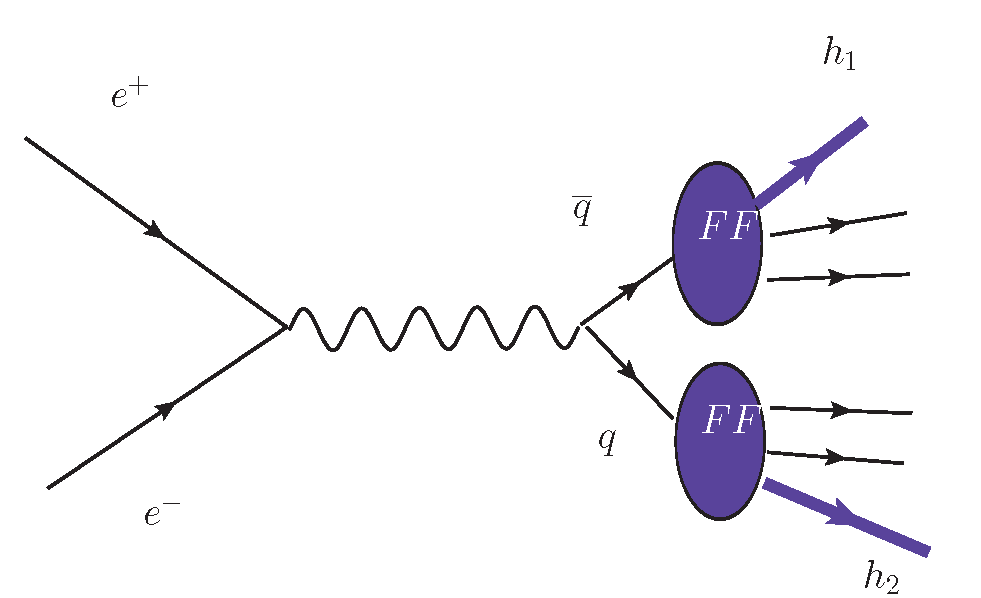
\includegraphics[width=0.8\textwidth,natwidth=610,natheight=642]{figure_theory/e+e-.png}
    \caption[Short caption]{The $e^+e^-$ annihilation process.}
    \label{fig:e+e-}
\end{figure}
The Collins mechanism describes the dependence of the transverse momentum of an unpolarized hadron on the transverse polarization of the parent quark. Here we define the transverse momentum with respect to the direction of the parent quark and call it $\boldsymbol{P}_{\bot}$, The transverse polarization of the transversely polarized quark is $\boldsymbol{S}_\perp$ and $\boldsymbol{k}$ is the momentum of the quark. The probability to find a hadron $h$ produced by a transversely polarized quark is\cite{ChargedPionResult,SSATrentoConvention}

\begin{equation}
D_{hq\uparrow}=D^q_1(z,P^2_{\bot})+H^{\bot q}_1(z,P^2_{\bot})\frac{(\hat{k}\times \boldsymbol{P}_{\bot})\cdot \boldsymbol{S}_{\perp}}{zM_h},
\label{eqn:FF1}
\end{equation}


In $e^+e^-\rightarrow q \bar q$  with unpolarized lepton lepton beams, we cannot measure a Collins effect in a single hemisphere, since we do not know the polarization of the parent quark. 
However, as shown in Fig.~\ref{fig:e+e-}, we can use the measurement of back-to-back hadrons, where the hadrons are detected in opposite hemispheres. In this case the correlation between the polarizations of the parent $q \bar q$ pair remains in the correlation of the Collins effects of $h_1$ and $h_2$~\cite{BoerThesis,ChargedPionResult2}. A naive picture is to think about the Collins effect as a left/right asymmetry. If we detect hadrons approximately perpendicular to the beam axis, we know that the parent quark was transversely polarized, but we don't know the direction. However, if we detect a hadron in the opposite hemisphere, we can measure the relative effect to that hadron which comes from quark with correlated polarization.

\subsubsection{Cross-section and Azimuthal Asymmetry in $e^+e^-$ Annihilation}

\begin{figure}[H]
  \centering     
  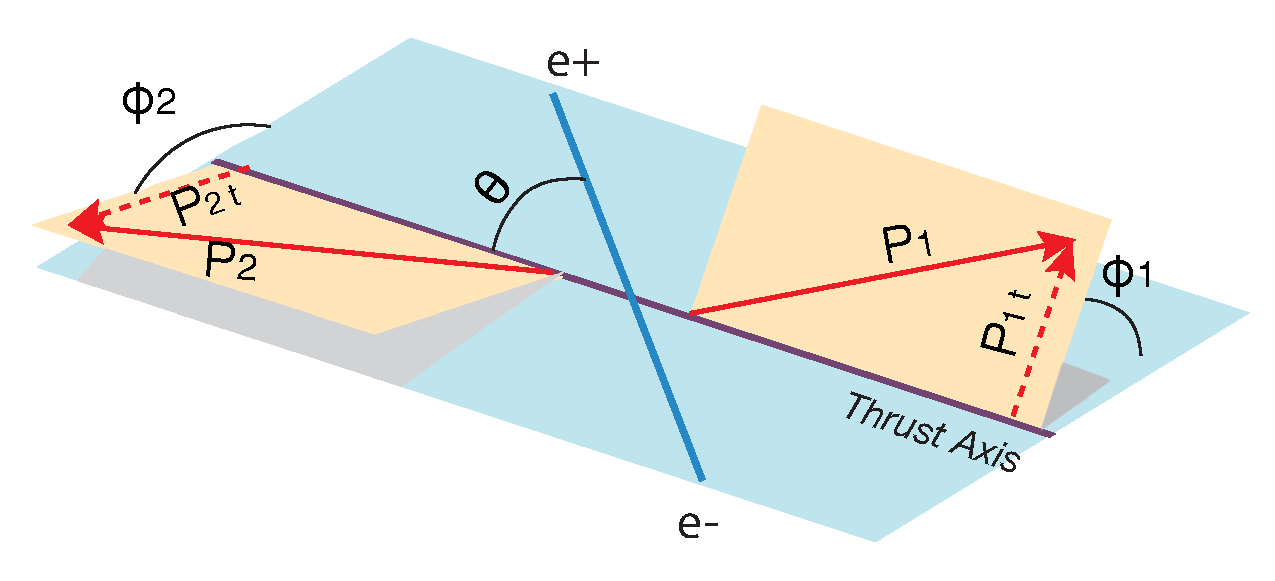
\includegraphics[width=.9\textwidth,natwidth=600,natheight=400]{figure_theory/e+e-_phi1phi2.pdf}
  \caption{Thrust reference frame.}
  \label{fig:phi1phi2frame}
\end{figure}

As discussed in~\cite{BoerThesis, Boer:2008fr}, the Collins effect in $e^+e^-$ can be measured in different frames which differ in the selection of the reference axis that is used to compute the azimuthal angles (For both frames the reference frame is the CMS). Either one chooses one of the hadrons ($h_1$) and measures the azimuthal angle of the other hadron around $h_1$, the so-called $\phi_0$ method, or one chooses the thrust axis of the event as the axis and measures the sum of the azimuthal angles $\phi_1$, $\phi_2$ of $h_1$ and $h_2$, respectively. This is sometimes called the $\phi_{12}$ method. We chose the later one. At leading order the thrust axis is connected to the unobserved $q \bar q$ axis, which connects this method to the naive description given earlier. It should be noted, that in previous measurements at Belle and BaBar, the thrust axis was corrected back to the $q \bar q$ axis from simulation. We do not do this for our analysis, since the matching to a leading order plus parton shower simulation is questionable, instead we will correct back to the true thrust axis to be defined later when we discuss the analysis.

Fig.~\ref{fig:phi1phi2frame} shows the frame that uses thrust axis as reference. The thrust axis~($\boldsymbol{\hat{n}}$) can be obtained by  maximizing:
\begin{equation}
\label{eq:thrust}
t=\sum_h\frac{|\boldsymbol{P_h\cdot\hat{n}}|}{|P_h|}.
\end{equation}
Here the summation runs over all stable final state particles. In experiment, not all final state particles can be collected thus the reconstructed thrust axis is not accurate. This effect will be discussed and corrected in subsection~\ref{sec:smearingcorrection}. 

In this reference frame, the differential cross-section is dependent on the fractional energies~($z_{1,2}$) and Collins angles~($\phi_{1,2}$) of hadron $h_{1,2}$ and expressed as~\cite{BoerThesis}:
\begin{equation}
\begin{aligned}
\frac{d\sigma(e^+e^-\rightarrow (\textrm{jet}+h_1)(\textrm{jet}+h_2)+X)}{d\Omega dz_1dz_2 d\boldsymbol{P}_{t1} d\boldsymbol{P}_{t2} d\phi_1d\phi_2}&\propto \\
\sum_{q,\bar{q}} \frac{3\alpha^2}{Q^2}\frac{e_q^2}{4}z^2_1z^2_2 \left\{ (1+\cos^2\theta)D_1^{q}(z_1,\boldsymbol{P}^2_{1\perp})\bar{D}_1^{\bar{q}}(z_2,\boldsymbol{P}^2_{2\perp})\right.\\  \left. +\sin^2\theta\cos(\phi_1+\phi_2)H_1^{\bot,q}(z_1,\boldsymbol{P}^2_{1\perp})\bar{H}_1^{\bot,\bar{q}}(z_2,\boldsymbol{P}^2_{2\perp})\right\},
\end{aligned}
\label{eqn:cross_subsection_ee}
\end{equation}
where the sum runs over all quark flavors accessible at the center-of-mass energy~\cite{BoerThesis}. In the leading order equation~\ref{eqn:cross_subsection_ee},  $\theta$ the angle between the colliding beam and the thrust axis.
The charge carried by each quark is written as $e_q$, $z_{1,2}$ and $\boldsymbol{P}_{1,2,\perp}$ are, as before, the fractional energies of the produced hadrons, $z_i\approx -\frac{2P_{i}\cdot q}{Q^2}=\frac{2*E_{h_i} }{\sqrt{s}}$,  and their transverse momentum with respect to $\boldsymbol{k}$. We call the observed transverse momentum of hadron $i$ with respect to the thrust axis $\boldsymbol{P}_{ti}$. In this work we extract the asymmetry using the leading order angular dependencies and substituting $\boldsymbol{P}_{ti}$ for $\boldsymbol{P}_{i\perp}$ and the thrust axis for the $q-\bar{q}$ axis. 

Equation.~\ref{eqn:cross_subsection_ee} can be written more compactly as:
\begin{equation}
d\sigma \sim A D_1^q \bar{D}_1^{\bar{q}}+B\cos(\phi_1+\phi_2)H^{\bot q}_{1}\bar{H}^{\bot \bar{q} }_{1}.
\label{eqn:FF2}
\end{equation}
\noindent where in Eq.~\eqref{eqn:FF2}, $A(y)=(\frac{1}{2}-y+y^2)$ and $B(y)=y(1-y)$. In the CMS, $A$ and $B$ can be described as $A(y)=\frac{1}{4}(1+\cos^2\theta)$ and $B(y)=\frac{1}{4}\sin^2\theta$. 

%Collins Fragmentation Function appears in the first order transverse moment as~\cite{AsyInPolarizedHadronProductionInEE}:
%\begin{equation}
%H_1^{\bot(1)}=z^2\int d^2 \boldsymbol{k}_T \frac{\boldsymbol{k}_T^2}{2M^2} H_1^{\bot}(z,z^2\boldsymbol{k}_T^2)
%\label{eqn:firstmomet}
%\end{equation}
%\noindent where $H^{\bot q}_1(z,P^2_{h\bot})$ is the Collins FF. Similarly with subsection~\ref{sec:SIDIScrosssubsection}, $z$ is defined as the fractional energy of the hadron $z\approx -\frac{2P_h\cdot q}{Q^2}=\frac{2*E_h}{\sqrt{S}}$. 
%The last item in Eq.~\eqref{eqn:FF1} is dependent on the quark spin direction and hence the transverse distribution function will lead to an asymmetric azimuthal angle distribution as shown in Eq.~\eqref{eqn:tssa}.   

\subsection{Observable}
\label{sec:observable}
A hadron pair is composed of hadrons $h_1$, $h_2$ from different hemispheres (back-to-back), which means for their respective three momenta $\boldsymbol{P}_{i}$:
\begin{equation}
(\boldsymbol{P}_{1} \cdot \hat{n})(\boldsymbol{P}_{2}\cdot \hat{n}) < 0 .
\end{equation}
If the two hadrons in different hemispheres are measured simultaneously, the Collins asymmetry will be proportional to $\cos(\phi_1+\phi_2)$. The angles $\phi_1$ and $\phi_2$ are shown in Fig.~\ref{fig:phi1phi2frame} and can be calculated using
\begin{equation}
%\phi_i=\frac{\hat{\boldsymbol{n}}}{|\hat{\boldsymbol{n}|}}\cdot(\frac{\hat{\boldsymbol{z}}\times\hat{\boldsymbol{n}}}{|\hat{\boldsymbol{z}}||\hat{\boldsymbol{n}}|}\times\frac{\hat{\boldsymbol{n}}\times\hat{\boldsymbol{P}_{h,i}}}{|\hat{\boldsymbol{n}}||\hat{\boldsymbol{P}_{h,i}}|})\arccos(\frac{\hat{\boldsymbol{z}}\times\hat{\boldsymbol{n}}}{|\hat{\boldsymbol{z}}||\hat{\boldsymbol{n}}|}\times\frac{\hat{\boldsymbol{n}}\times\hat{\boldsymbol{P}_{h,i}}}{|\hat{\boldsymbol{n}}||\hat{\boldsymbol{P}_{h,i}}|}),
\phi_i=sgn[\hat{\boldsymbol{n}}\cdot \{ (\boldsymbol{z}\times\hat{\boldsymbol{n}})\times(\hat{\boldsymbol{n}}\times{\boldsymbol{P}_{i}})\}]\times \arccos(\frac{\hat{\boldsymbol{z}}\times\hat{\boldsymbol{n}}}{|\hat{\boldsymbol{z}}\times\hat{\boldsymbol{n}}|}\times\frac{\hat{\boldsymbol{n}}\times{\boldsymbol{P}_{i}}}{|\hat{\boldsymbol{n}}\times{\boldsymbol{P}_{i}}|}),
\label{eqn:collinsangledefine2}
\end{equation}
here $i$ stands for the hadron from first or second hemisphere and $\boldsymbol{z}$ is the unit vector along the beam direction.

The Collins angle of a hadron pair is $\phi_{12} \equiv \phi_1+\phi_2$. The di-hadron yield $N_{12}=N_{12}(\phi_1+\phi_2)$ divided by the average yield gives the normalized rate $R_{12}=\nicefrac{N_{12}}{\langle  N_{12}\rangle}$. Considering the $\cos(\phi_1+\phi_2)$ modulation, $R_{12}$ can be parameterized as $R_{12}=a_{12}(\theta,z_1,z_2, \boldsymbol{P}^2_{h1\bot},\boldsymbol{P}^2_{2\bot})\cos(\phi_1+\phi_2)+b_{12}$ with the azimuthal asymmetry
\begin{equation}
a_{12}(\theta,z_1,z_2, \boldsymbol{P}^2_{t1},\boldsymbol{P}^2_{t2})=\frac{\sin^2\theta}{1+\cos^2\theta}
\frac{\sum\limits_{q}e^2_qH^{\bot q}_1(z_1,\boldsymbol{P}^2_{t1})\bar{H}^{\bot q}_1(z_2,\boldsymbol{P}^2_{t2})}{\sum\limits_{q}e^2_qD^q_1(z_1,\boldsymbol{P}^2_{t1})\bar{D}^{\bar{q}}_1(z_2,\boldsymbol{P}^2_{t2})}.
\end{equation} 
Here $b_{12}$ is the normalized yield which should be consistent with 1.
Note that in the equation for $a_{12}$ above, we kept the full dependence of the asymmetry $a_{12}$ on the $z_i$ and $ \boldsymbol{P}^2_{ti}$. In the measurements presented later in the note, we keep at most two variables differential, the other ones are integrated out (There is no convolution over the transverse momenta since this is the thrust method, not the $\phi_0$ method).
As will be discussed later (see subsection~\ref{sec:dataselection}), the azimuthal distribution can be strongly distorted due to acceptance effects. Furthermore, initial-state radiation (ISR) and gluon radiation introduce cosine modulations similar to the ones arising from the Collins effect. To remedy those effects the double ratio (DR) method, in which we calculate the ratio of normalized distribution between certain different kinds of hadron pairs, can be used as the effects are assumed to be charge independent and thus largely cancel during the ratio calculation~\cite{ChargedPionResult,CollinsInSIDISandEE}.  For example, in the charged pion analysis, the double ratio was designed to be the ratio of unlike sign pairs ($\pi^+\pi^-$) to like sign pairs ($\pi^+\pi^+$ and $\pi^-\pi^-$).


In this note, double ratios for neutral mesons are designated as:
\begin{equation}
\label{eqn:FF6}
\begin{aligned}
A_{12}^{\pi^0}=\frac{A^{0\pm}_{12}}{A^L_{12}}=\frac{\pi^0\pi^++\pi^0\pi^-}{\pi^+\pi^++\pi^-\pi^-}\\
A_{12}^{\eta}=\frac{A^{\eta\pm}_{12}}{A^L_{12}}=\frac{\eta\pi^++\eta\pi^-}{\pi^+\pi^++\pi^-\pi^-}.
\end{aligned}
\end{equation}
For charged pions we can consider asymmetries of likesign pairs (L), unlikesign pairs (U) or pairs that are integrated over both charges (C).
With these we can construct three more double ratios:

\begin{equation}
\label{eqn:FF7}
\begin{aligned}
A_{12}^{UL}=\frac{A^{U}_{12}}{A^L_{12}}=\frac{\pi^+\pi^-+\pi^-\pi^+}{\pi^+\pi^++\pi^-\pi^-}\\
A_{12}^{UC}=\frac{A^{U}_{12}}{A^C_{12}}=\frac{\pi^+\pi^-+\pi^-\pi^+}{\pi^+\pi^++\pi^-\pi^-+\pi^+\pi^-+\pi^-\pi^+}\\
A_{12}^{UC}=\frac{A^{U}_{12}}{A^C_{12}}=\frac{\pi^+\pi^++\pi^-\pi^-+\pi^+\pi^-+\pi^-\pi^+}{\pi^+\pi^++\pi^-\pi^-}.
\end{aligned}
\end{equation}


The asymmetry $A^C$ is thought to be related to the asymmetries involving $\pi^0$'s, therefore the double ratio $A_{12}^{CL}$ should be equal to $A_{12}^{\pi^0}$~\cite{Efremov:2006qm}, 
which we will test with the experimental data.
%For the Collins effect, the Collins FF can be separated into favored and unfavored parts according to which flavor goes into the hadron where charge-conjugation and isospin symmetry arguments have been used~\cite{CollinsInSIDISandEE}:


Fragmentation functions are often categorized into favored and disfavored ones, depending on whether or not the fragmenting-quark flavor is part of the valence structure of the hadron formed. For charged pions, employing charge-symmetry and isospin asymmetry, FFs are 
\begin{equation}
\begin{aligned}
D^{fav}=D^{u/{\pi^+}}=D^{d/{\pi^-}}=D^{\bar{u}/{\pi^-}}=D^{\bar{d}/{\pi^+}}\\
D^{dis}=D^{u/{\pi^-}}=D^{d/{\pi^+}}=D^{\bar{u}/{\pi^+}}=D^{\bar{d}/{\pi^-}}.
\label{eqn:FF4}
\end{aligned}
\end{equation}
The fragmentation functions of $\pi^0$ consist of both favored and disfavored FFs~\cite{FoundationsofpQCD,Efremov:2006qm},
\begin{equation}
\begin{aligned}
D^{u/{\pi^0}}=D^{\bar{u}/{\pi^0}}=D^{d/{\pi^0}}=D^{\bar{d}/{\pi^0}}=\frac{1}{2}(D^{dis}+D^{fav}).
\label{eqn:FF4pi0}
\end{aligned}
\end{equation}
Besides light quarks, we also consider the contribution of strange quarks.
% A common assumption is that the probability for strange-quark fragments into charged pions is the same as the light-quark disfavored ones, as it also requires generating the two valence quarks forming the pion, thus
A common assumption is that the probability for strange-quark fragmentation is the same for all pion states, thus
\begin{equation}
D^{dis}_{s\rightarrow\pi}=D^{s/{\pi^-}}=D^{s/{\pi^+}}=D^{s/{\pi^0}}.
\end{equation}

Asymmetries after applying the double ratio, for instance, like sign pairs $A^L_{12}$ and $\pi^0\pi^{\pm}$ pairs $A^{0\pm}_{12}$, can be expressed in terms of various FFs~\cite{Efremov:2006qm}:

\begin{multline}
A_{12}^{\pi^0}=\frac{A^{0\pm}_{12}}{A^L_{12}}=1+\cos(\phi_1+\phi_2)\frac{\sin^2(\theta)}{1+\cos^2(\theta)} \\
\times\bigg\{\frac{5(H^{\bot,fav}_1+H^{\bot,dis}_1)(H^{\bot,dis}_1+H^{\bot,fav}_1)+4H^{\bot,dis}_{1,s\rightarrow\pi}H^{\bot,dis}_{1,s\rightarrow\pi}}{5(D^{\bot,fav}_1+D^{\bot,dis}_1)(D^{\bot,dis}_1+D^{\bot,fav}_1)+4D^{dis}_{1,s\rightarrow\pi}D^{dis}_{1,s\rightarrow\pi})}\\
-\frac{5H^{\bot,fav}_1H^{\bot,dis}_1+5H^{\bot,dis}_1H^{\bot,fav}_1+2H^{\bot,dis}_{1,s\rightarrow\pi}H^{\bot,dis}_{1,s\rightarrow\pi}}{5D^{\bot,fav}_1D^{\bot,dis}_1+5D^{\bot,dis}_1D^{\bot,fav}_1+2D^{dis}_{1,s\rightarrow\pi}D^{dis}_{1,s\rightarrow\pi}} \bigg\}.
\label{eqn:FF5}
\end{multline}
%Due to the differing valence structure of the $\eta$, the FFs composition the relations above~\ref{eqn:FF5} read differently:

To study the FFs expression of $\eta$, due to the different valence structure with $\pi^0$, we need to reconsider the cases with strange-quark fragments into $\eta$. 
\begin{equation}
\begin{aligned}
D^{u/{\eta}}=D^{d/{\eta}}=D^{\bar{u}/{\eta}}=D^{\bar{d}/{\eta}}=\frac{1}{2}\left(D^{fav_\eta}+D^{dis_\eta}\right).
\label{eqn:FFetaquark}
\end{aligned}
\end{equation}

%Neglecting symmetry breaking due to strangeness suppression, the strange-quark FFs can be related to the non-strange ones:
%\begin{equation}
%\begin{aligned}
%D^{s/{\eta}}=D^{\bar{s}/{\eta}}=\frac{1}{2}\left(D^{fav_\eta}+D^{dis_\eta}\right).`
%\end{aligned}
%\end{equation}
%However, here we do not use this relation. 
Using~\ref{eqn:FFetaquark} results in the following expression for the double ratio:
\begin{multline}
A_{12}^{\eta}=\frac{A^{\eta\pm}_{12}}{A^L_{12}}=1+\cos(\phi_1+\phi_2)\frac{\sin^2(\theta)}{1+\cos^2(\theta)} \\
\times\bigg\{\frac{5(H^{\bot,fav_\eta}_1+H^{\bot,dis_\eta}_1)(H^{\bot,dis}_1+H^{\bot,fav}_1)+2(H^{\bot,fav}_{1,s\rightarrow\eta}+H^{\bot,dis}_{1,s\rightarrow\eta})H^{\bot,dis}_{1,s\rightarrow\pi}}{5(D^{\bot,fav_\eta}_1+D^{\bot,dis_\eta}_1)(D^{\bot,dis}_1+D^{\bot,fav}_1)+2(D^{dis}_{1,s\rightarrow\eta}+D^{dis}_{1,s\rightarrow\eta})D^{dis}_{1,s\rightarrow\pi})}\\
-\frac{5H^{\bot,fav}_1H^{\bot,dis}_1+5H^{\bot,dis}_1H^{\bot,fav}_1+2H^{\bot,dis}_{1,s\rightarrow\pi}H^{\bot,dis}_{1,s\rightarrow\pi}}{5D^{\bot,fav}_1D^{\bot,dis}_1+5D^{\bot,dis}_1D^{\bot,fav}_1+2D^{dis}_{1,s\rightarrow\pi}D^{dis}_{1,s\rightarrow\pi}} \bigg\}.
\label{eqn:FF5eta}
\end{multline}

The parameterization $A_{12}*\cos(\phi_1+\phi_2)$ is fitted to the final double ratio distribution, where the amplitude $A_{12}$ is the azimuthal asymmetry that is measured in this note. 